\documentclass[tikz,border=8pt]{standalone}
\usepackage{amsmath,amssymb}
\usetikzlibrary{arrows.meta,automata,positioning,quotes}
\begin{document}
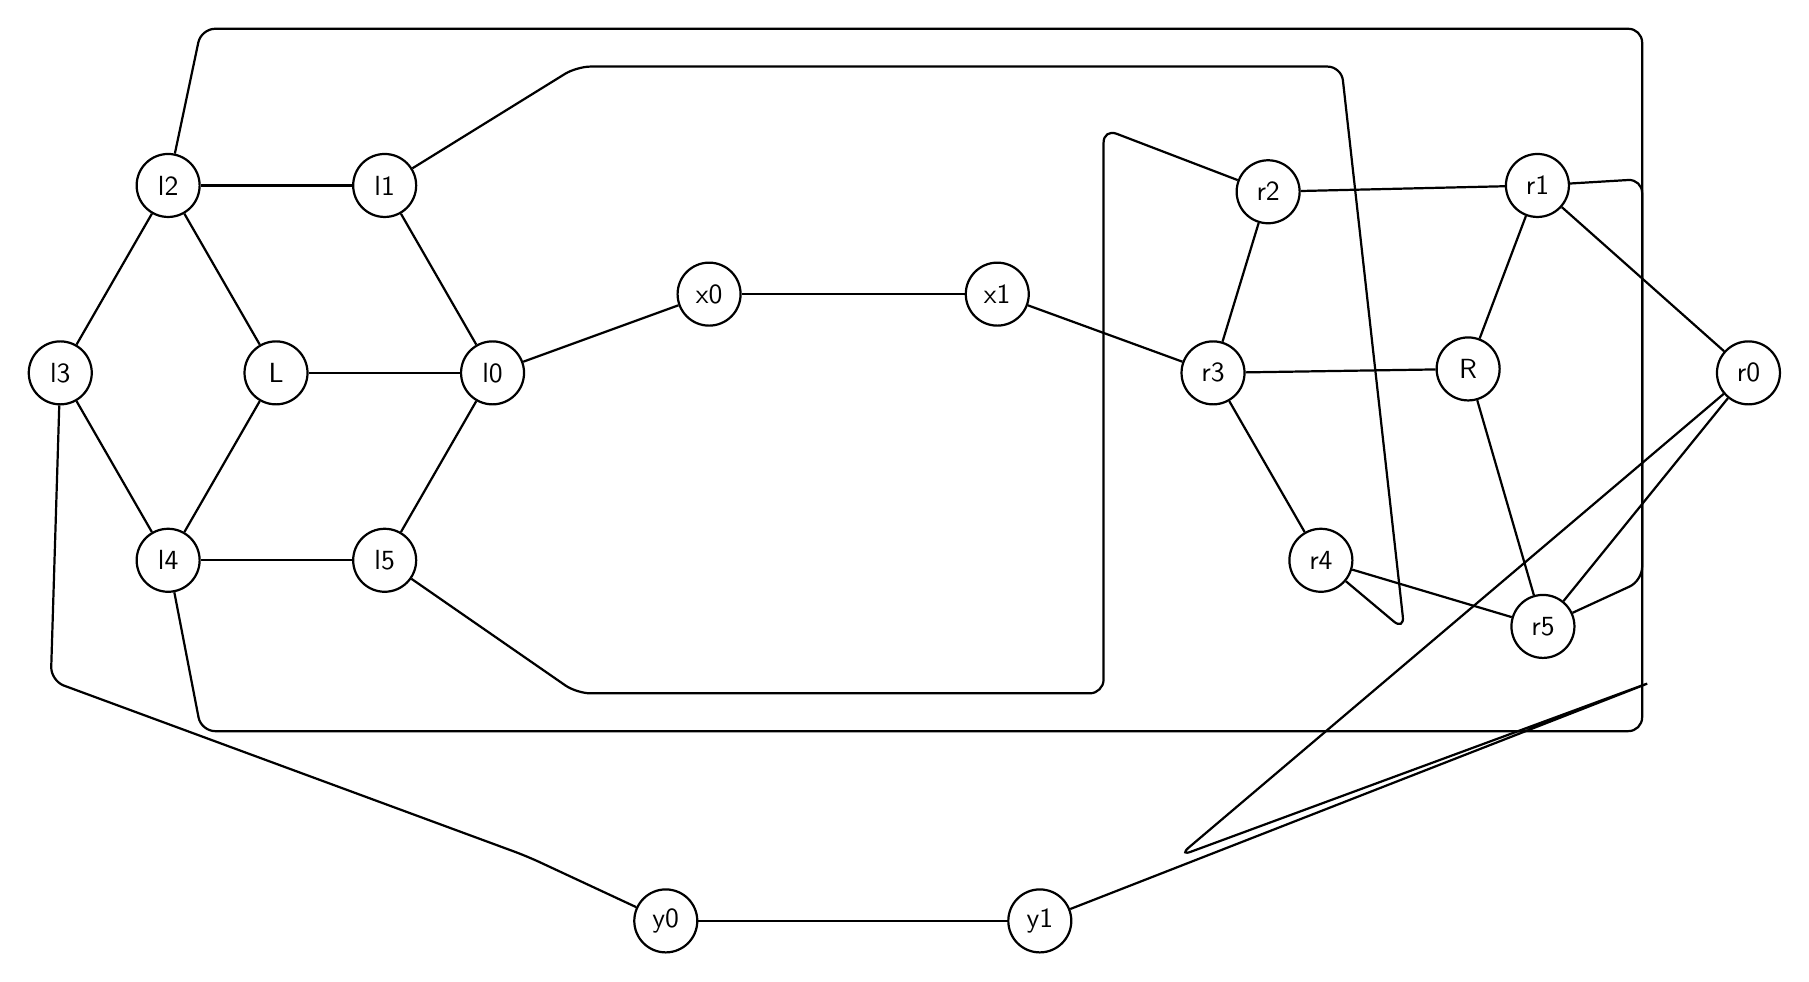
\begin{tikzpicture}[x=1cm,y=1cm]
\tikzset{
  graphnode/.style={circle,draw,thick,minimum size=8mm,inner sep=1pt,font=\sffamily},
  directed/.style={-{Stealth[length=2.4mm]},thick},
  undirected/.style={thick}
}
\node[graphnode] (n_L) at (-7.35,0.32) {L};
\node[graphnode] (n_l0) at (-4.60,0.32) {l0};
\node[graphnode] (n_l1) at (-5.97,2.70) {l1};
\node[graphnode] (n_l2) at (-8.72,2.70) {l2};
\node[graphnode] (n_l3) at (-10.09,0.32) {l3};
\node[graphnode] (n_l4) at (-8.72,-2.06) {l4};
\node[graphnode] (n_l5) at (-5.97,-2.06) {l5};
\node[graphnode] (n_R) at (7.79,0.37) {R};
\node[graphnode] (n_r0) at (11.35,0.32) {r0};
\node[graphnode] (n_r1) at (8.67,2.70) {r1};
\node[graphnode] (n_r2) at (5.25,2.62) {r2};
\node[graphnode] (n_r3) at (4.55,0.32) {r3};
\node[graphnode] (n_r4) at (5.92,-2.06) {r4};
\node[graphnode] (n_r5) at (8.74,-2.90) {r5};
\node[graphnode] (n_x0) at (-1.85,1.32) {x0};
\node[graphnode] (n_x1) at (1.81,1.32) {x1};
\node[graphnode] (n_y0) at (-2.40,-6.64) {y0};
\node[graphnode] (n_y1) at (2.35,-6.64) {y1};
\draw[undirected] (n_l0) -- (n_l1);
\draw[undirected] (n_l1) -- (n_l2);
\draw[undirected] (n_l2) -- (n_l3);
\draw[undirected] (n_l3) -- (n_l4);
\draw[undirected] (n_l4) -- (n_l5);
\draw[undirected] (n_l5) -- (n_l0);
\draw[undirected] (n_L) -- (n_l0);
\draw[undirected] (n_L) -- (n_l2);
\draw[undirected] (n_L) -- (n_l4);
\draw[undirected] (n_r0) -- (n_r1);
\draw[undirected] (n_r1) -- (n_r2);
\draw[undirected] (n_r2) -- (n_r3);
\draw[undirected] (n_r3) -- (n_r4);
\draw[undirected] (n_r4) -- (n_r5);
\draw[undirected] (n_r5) -- (n_r0);
\draw[undirected] (n_R) -- (n_r1);
\draw[undirected] (n_R) -- (n_r3);
\draw[undirected] (n_R) -- (n_r5);
\draw[undirected] (n_l0) -- (n_x0);
\draw[undirected] (n_x0) -- (n_x1);
\draw[undirected] (n_x1) -- (n_r3);
\draw[undirected,rounded corners=5pt] (n_l3) -- (-10.21,-3.59) -- (-4.16,-5.82) -- (n_y0);
\draw[undirected] (n_y0) -- (n_y1);
\draw[undirected,rounded corners=5pt] (n_y1) -- (10.16,-3.59) -- (4.11,-5.82) -- (n_r0);
\draw[undirected,rounded corners=5pt] (n_l1) -- (-3.53,4.21) -- (6.18,4.21) -- (6.98,-2.95) -- (n_r4);
\draw[undirected,rounded corners=5pt] (n_l2) -- (-8.30,4.69) -- (10.00,4.69) -- (10.00,-2.32) -- (n_r5);
\draw[undirected,rounded corners=5pt] (n_l4) -- (-8.30,-4.23) -- (10.00,-4.23) -- (10.00,2.78) -- (n_r1);
\draw[undirected,rounded corners=5pt] (n_l5) -- (-3.53,-3.75) -- (3.16,-3.75) -- (3.16,3.42) -- (n_r2);
\end{tikzpicture}
\end{document}
